\chapter{Progettazione e Realizzazione di un Ambiente per la Configurazione Avanzata}\label{capitolo:progettazione_realizzazione}
\markboth{Progettazione e Realizzazione}{}
Questo capitolo è dedicato alla comprensione e descrizione delle fasi di progettazione e realizzazione di \visualnetkit{}. Si mostretà in maniera dettagliata la nuova struttura dei \plugin{} accennata nel precedente capitolo, e successivamente verrà mostrato il resto del sistema analizzando i singoli moduli che lo compongono.

\begin{figure}[!htb]
	\centering
	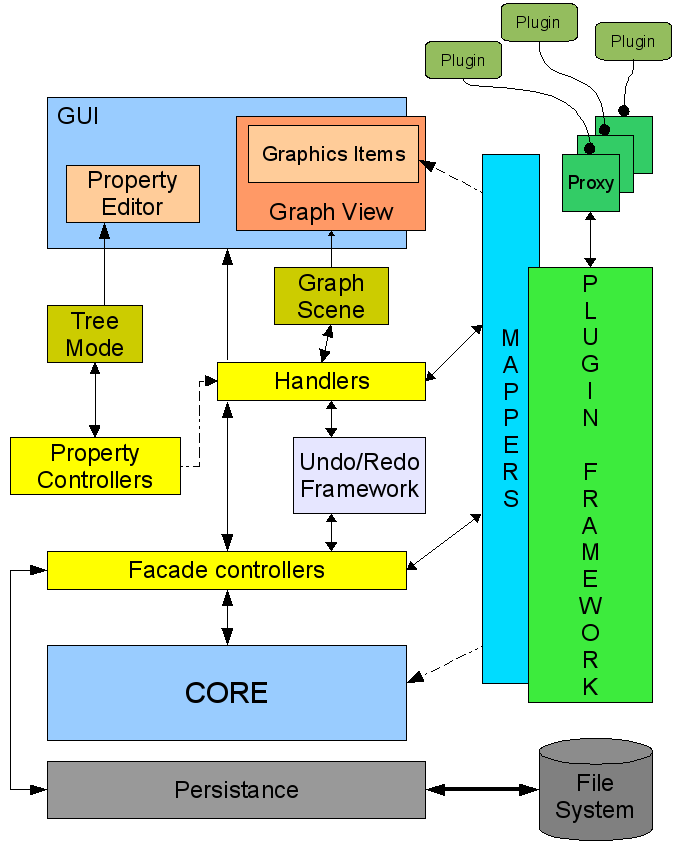
\includegraphics[width=8cm]{images/diagramma_componenti_vnetkit.png}
	\caption{Diagramma dei componenti di \visualnetkit{}}
	\label{figura:vn_componenti}
\end{figure}

In questa introduzione vogliamo subito dare al lettore un quadro generale (figura \ref{figura:vn_componenti}) della composizione architetturale nello stato attuale di \visualnetkit{}, in modo da rendere più facile la localizzazione degli elementi durante la loro trattazione.

\section{Architettura modulare basata su \plugin{}}
Come primo argomento vogliamo concentrarci sulla trattazione della struttura modulare di \visualnetkit{}, che rappresenta anche il suo punto di forza in ambito di flessibilità ed estendibilità. 

Può essere auspicabile che un software pur uso in ambito scientifico sia in possesso di funzionalità opzionali, vale a dire funzionalità che possono essere aggiunte o rimosse nel corso di una simulazione senza grossi ostacoli. Per esempio, si pensi a quanto può essere utile ad un progettista osservare il comportamento di una rete con o senza un tederminato servizio (ad esempio \emph{IPv6}) sulle macchine di cui è composta, o per uno studente quanto risulti comprensibile studiare una topologia di rete malleabile che si presta a tutti i possibili test che egli vuol effettuare.

L'utilizzo di un'architettura basata su \plugin{} dona grande flessibilità all'intero sistema ed in particolare agli utenti finali.

\subsubsection{Perché un sistema basato su \plugin{}?}
Durante le prime iterazioni e le prime fasi di testing emersero alcuni fattori di alto rischio; l'architettura era stata concepita e realizzata basandosi fortemente sul concetto che tutti i requisitivi dovevano essere assemblati staticamente nell'applicazione (come accade nei vari ambienti di configurazioni descritti nella sezione \ref{subsection:ccrc}).

Questa scelta prevedeva una lunghissima fase di sviluppo ed una continua ricerca e specifica dei requisiti e dei casi d'uso che avrebbero potuto destabilizzare l'intero sistema. Inoltre adottando questa tecnica non si sarebbe mai riusciti ad offrire una totale elasticità, ma piuttosto si sarebbe dovuto scendere a compromessi su cosa implementare e cosa no.

Analizzando meglio gli obiettivi si è giusti alla conclusione che l'unica strada percorribile fosse quella che prevedeva la trasformazione dell'architettura in una modularizzata. Il core del sistema (senza alcun \plugin{} attivo) avrebbe offerto all'utente solamente la possibilità di creare una rete a livello topologico, priva quindi di caratteristiche proprie.

Questa nuova tecnica avrebbe da un lato offerto una sicura controllabilità dei fattori di rischio, restringendoli alla re-ingegnerizzazione del sistema per renderlo modulare, dall'altro avrebbe reso \visualnetkit{} estremamente scalabile e flessibile e gli avrebbe conferito una connotazione del tutto unica nel suo genere.

\subsection{Interazione tra sistema e \plugin{}}
Quando si sviluppa un'applicazione che si basa fortemente su \plugin{} la cosa più importante è definire i confini dell'uno e dell'altro sistema. In poche parole ambiente e moduli devono essere ben descritti per non imbattersi in fenomei di sovrapposizione; questi due mondi devono cooperare, ma non devono intralciarsi né tantomeno svolgere le stesse mansioni.

Dopo un'attenta ed accurata fase di studio si è arrivati a definire la linea di demarcazione tra il sistema e le estensioni. I vari \plugin{} possono essere attivati sugli elementi di base del sistema offrendo una sorta di caratterizzazione più specifica. Su di un elemento possono essere attivi contemporaneamente più \plugin{} che di fatto donano una definizione ben precisa all'elemento. Se per esempio su un host noi attiviamo \plugin{} quali DNS e HTTP, balza subito all'occhio il tipo di quell'oggetto; abbiamo semplicemente di fronte una macchina virtuale che offre un servizio di DNS e che allo stesso tempo è un server Web di qualche tipo.

Andiamo ora a descrivere in dettaglio la struttura del sotto sistema che permette ai moduli di colloquiare con il core dell'applicazione e la definizione delle varie interfaccie - figura \ref{figura:uml_plugin_framework}.

\begin{figure}[!htb]
	\centering
	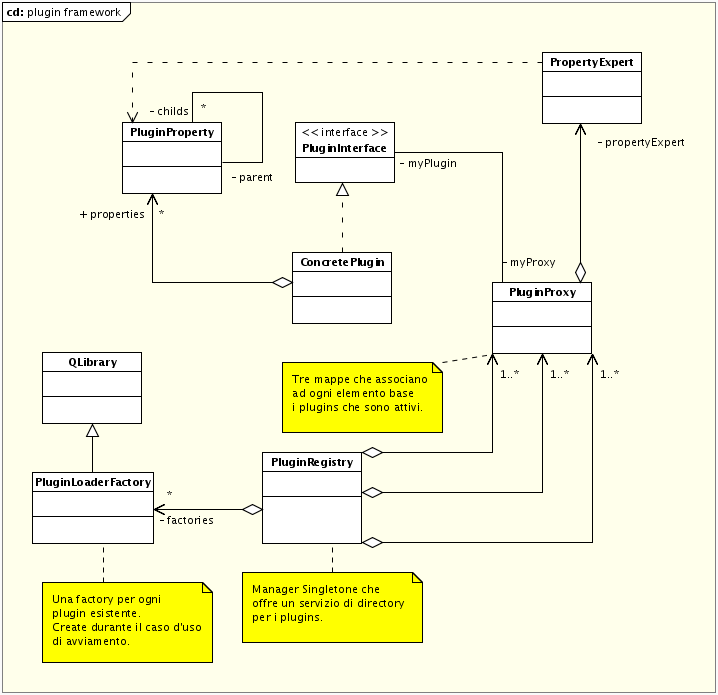
\includegraphics[width=12cm]{images/plugin_framework_uml.png}
	\caption{Diagramma delle classi del sotto sistema di gestione dei \plugin{}.}
	\label{figura:uml_plugin_framework}
\end{figure}

Com'è facile osservare, tutto ruota intorno alla classe singletone ``PluginRegistry''. Questo controller viene invocato dal sistema nel caso d'uso d'avviamento per fetchare i \plugin{} esistenti, validarli e creare per ognuno di questi il proprio loader factory. Il PluginRegistry offre un servizio di directory, ossia è quel componente che mantiene traccia delle associazioni tra un \plugin{} e un elemento base.

In realtà il sistema non conosce l'instanza di un determinato modulo direttamente, ma conosce il suo \proxy{} che introduce un livello di indirezione tra il sistema e il \plugin{} stesso. La scelta di applicare il pattern \proxy{} assicura un buon controllo d'accesso all'oggetto reale di cui è responsabile e permette inoltre un accesso trasparente verso il sistema. Analizziamo ora la classe astratta pura PluginInterface:
\begin{lstlisting}
/**
 * PluginInterface.h
 */
class PluginInterface
{
public:
	virtual ~PluginInterface() {};

	virtual bool saveProperty(QString propUniqueId, QString propValue,
			QString *pluginAlertMsg = NULL) = 0;

	virtual QString getXMLResource() = 0;

	virtual QMap<QString, QString> getTemplates() = 0;
	
	virtual QList<PluginProperty*> getPluginProperties() = 0;

	virtual PluginProxy* getProxy() = 0;

	virtual void setProxy(PluginProxy* p) = 0;

	virtual void setGroupID(qint32 id) { Q_UNUSED(id) };
	virtual qint32 getGroupID() { return -1; };

	virtual QString getDefaultGraphisLabel() = 0;

	virtual QString getName() = 0;

	virtual bool init(QString laboratoryPath) = 0;
	
	virtual QString deleteProperty(QString propertyUniqueId) = 0;
	
	virtual QPair<PluginProperty*, QString> addProperty(
		QString propertyIdToAdd, QString parentPropertyUniqueId) = 0;
	
};

typedef PluginInterface* createPlugin_t();
typedef void destroyPlugin_t(PluginInterface*);
\end{lstlisting}

Le più importanti righe di codice di questa classe sono gli ultimi due ``typedef''. Ogni implementazione di un \plugin{} deve necessariamente avere al suo interno definite le factory di creazione e discruzione definite come \emph{extern ``C''}. Queste due funzioni sono usate dalla classe LoaderFactory (che risolve i due simboli \textbf{createPlugin} e \textbf{destroyPlugin}) che permettono di creare nuove instanze di un determinato modulo. Un tipico esempio nell'uso di queste due funzioni è riportato qui di seguito:

\begin{lstlisting}
/* Factory (creator) */
extern "C" PluginInterface* createPlugin()
{
	return new YourContretePluginClass();
}

/* Factory (destroyer) */
extern "C" void destroyPlugin(PluginInterface* p)
{
	delete p;
}
\end{lstlisting}
Per avere informazioni aggiuntive su come creare un \plugin{}, si legga l'appendice A.

Ogni modulo è descritto da un proprio file di configurazione scritto in \xml{} che deve necessariamente essere inserito all'interno del \emph{Qt Resource System}\footnote{Il sistema di risolse di \qt{} consiste in un metodo (platform-indipendent) per la memorizzazione di file binari all'interno dell'applicazione stessa. Questa è una tecnica molto utile se l'applicazione ha sempre bisogno di determinati files e non si vuole correre il rischio di non possederli a runtime.}. All'interno di questo file vi sono descritte le credenziali del \plugin{} come il nome, descrizione, autori, dipendenze ecc\ldots, ma anche un'accurata descrizione delle proprietà offerte all'elemento a cui verrà attivato.

Per facilitare tutto questo ogni \proxy{} è equipaggiato di una classe expert che si occupa della validazione e interrogazione del file \xml{} pocanzi citato, nonché della manipolazione delle properties (poste all'interno di una struttura ad alberi n-ari).

Il sotto sistema appena descritto offre la possibilità di estendere le funzionalità di \visualnetkit{}. I vari \plugin{} sono elementi passivi che vengono invocati dal sistema quando necessario: l'utente agisce su una property, l'utente inizializza un \plugin{}, ecc\ldots Tuttavia un modulo può anche interagire con il sistema stesso ma solamente dopo che è stato invocato; in particolare durante la fase di inizializzazione il sistema chiama le funzioni di ``getXmlResource()'' e ``getDefaultGraphisLabel()'' per validare e scrivere una label nella vista del grafo della rete.

Si è voluti iniziare latrattazione dei componneti dell'architettura di \visualnetkit{} proprio dal sistema modulare su cui si basa, poiché si ritiene che questa parte è la più innovativa e non è presente in nessuno degli ambienti grafici sperimentati.

\section{Elementi architetturali}
Accurato il funzionamento e la logica che risiede dietro il framework dei \plugin{}, possiamo iniziare a introdurre gli altri elementi architetturali che di fatto supportano e interagiscono l'un l'altro per soddisfare tutti i requisiti (funzionali e non) che il sistema possiede.

Si inizierà ad analizzare gli elementi in figura \ref{figura:vn_componenti} con strategia \textbf{top-down} per quanto riguarda gli elementi a struttura orizzontale, poi si analizzeranno ai mappers ed in fine gli sforzi verranno convogliati nella descrizione del nuovo sitema che offre ai \plugin{} la possibilità di possedere un alta dinamicità nelle proprietà che essi offrono.

\subsection{L'interfaccia utente}
Uno degli obiettivi principali di questo progetto è la realizzazione di un ambiente di configurazione di reti virtuali che offra un'interfaccia grafica capace di fornire una vista intuitiva della rete virtuale  e permette di interagire in modo semplice con lo strato di emulazione offerto da \netkit{}.
Tale interfaccia, oltre a garantire un alto livello di ergonomia e usabilità, deve garantire buone capacità di adattamento al variare dei requisiti.

Sebbene la realizzazione di una interfaccia grafica possa dare l'impressione di essere un'attività semplice, durante tale periodo si incontrano svariate difficoltà in quanto l'ambiente in esame si avvicina molto alla definizione di ``IDE''\footnote{Un \textit{integrated development environment} (IDE), in italiano ambiente integrato di sviluppo, è un software che aiuta i programmatori nello sviluppo del software.} orientato - nel nostro caso - allo sviluppo di reti virtuali.

La realizzazione dell'attuale interfaccia ha richisto diversi cicli di sviluppo e raffinamento per ottenere un risultato apprezzabile e intuitivo. Questa è composta da varie \emph{docks} che al loro interno contengono vari sotto elementi come properties, zoom e miniatura del grafo, elementi attivi, struttura de lab e un elemento centrale che rappresenta la scena, ossia l'ambiente per disegnare la topologia di rete desiderata. L'ampio uso di grafica SVG fa si che all'utente arrivi subito un feedback positivo che incentiva lo stesso a sperimentare le caratteristiche offerte dall'ambiente che ha davanti.

Il grafo non è altro che l'elemento vista della struttura del modello di dominio; per ogni elemento grafico (Hosts, Collision Domains, Links) esiste un elemento di basso livello associato che incapsula le informazioni. Gli elementi grafici sono sostanzialmente degli oggetti che riflettono queste informazioni all'utente e gli consentono di interagire con gli elementi stessi.

L'esistenza del \emph{Graphics View Framework} offerto da \qt{}, ha reso minimi gli sforsi implementativi in quanto questo è fortemente basato sul pattern MVC che consente di collegare uno stesso modello (la scena) a più viste come avviene per la scena e la dock della miniatura - figura \ref{figura:vnetkit_graphics_view_1}.

\begin{figure}[!htb]
	\centering
	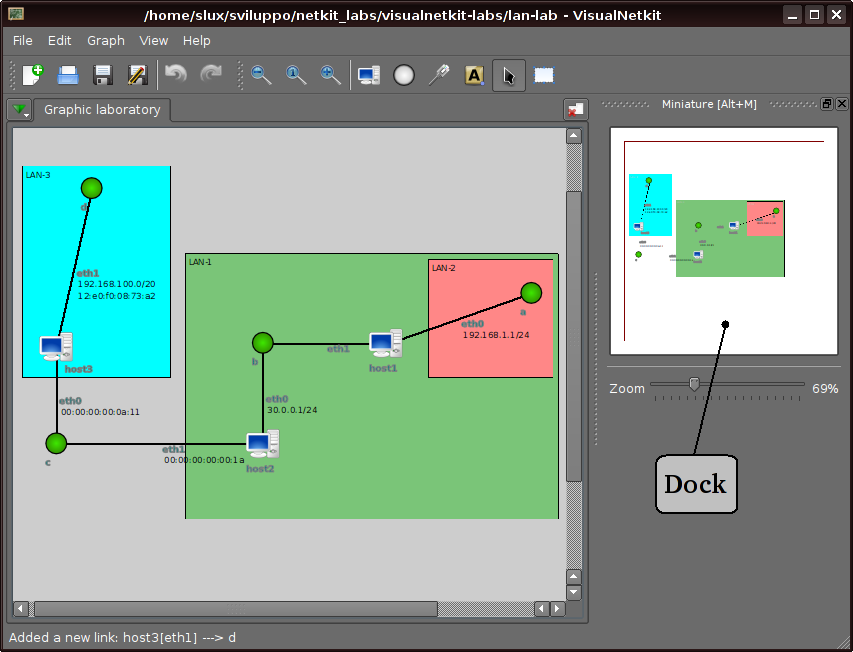
\includegraphics[width=12cm]{images/visualnetkit_graphics_view_1.png}
	\caption{Scena del grafo inserita in due viste differenti.}
	\label{figura:vnetkit_graphics_view_1}
\end{figure}

\subsubsection*{Dettagli implementativi}
La parte che riguarda l'interazione con l'utente è stata implementata seguendo i principi dell'\emph{event driven programming}, che rappresenta la base della programmazione delle interfacce grafiche. La programmazione guidata dagli eventi non considera i meccanismi standard di input (ad esempio la CLI - \emph{Command Line Interface}) ma basa il suo funzionamento sulla gestione degli eventi generati dall'utente, coma la pressione di un bottone, di un click del mouse. 

L'insieme degli eventi considerati interessati, vengono ricevuti da handlers che effettuano una prima validazione e inoltrano lo stesso evento agli strati di competenza posti solitamente a strati più bassi.

\subsubsection*{Signals e Slots in \qt{}}
In \qt{} slot e segnali sono usati per la comunicazione asincrona tra oggetti.
Si vuole che oggetti di un certo tipo vengano avvertiti e siano in grado di comunicare con altri oggetti quando su di un oggetto si scatena un determinato evento. Per esempio quando un utente clicka un bottone \textbf{Close}, probabilmente vorremmo che il widget si chiuda chiamando la sua funzione ``close''.

Un segnale viene emesso quando un particolare evento accade; uno slot invece è una funzione che se invocata è responsabile di gestire un particolare segnale ma può anche essere invocata in maniera sincrona da un qualche oggetto.

Tale meccanismo nasconde in realtà un sistema già noto con il nome di pattern Observer; l'unica differenza risiede nelle chiamate asincrone che i signal effettuano allo slot di loro competenza, senza aspettare una risposta. Infatti, ogni slot è definito con un tipo di ritorno ``void'' e l'unico che uno slot ha di effettuare modifiche è tramite effetti collaterali sull'elemento passato come puntatore. In figura \ref{figura:qt_signals_slots} è mostrato un esempio d'uso di Signals e Slots.

\begin{figure}[!htb]
	\centering
	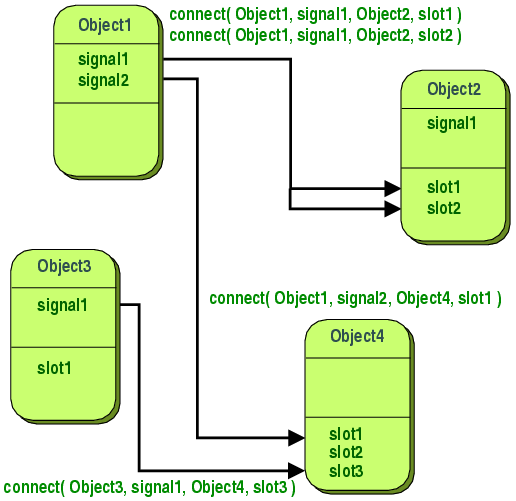
\includegraphics[width=8cm]{images/signals_slots.png}
	\caption{Schema d'uso di Signals e Slots.}
	\label{figura:qt_signals_slots}
\end{figure}

\subsection{Elementi del dominio}
Il kernel di questo progetto è il primo componente che è stato sviluppato ed anche il più importante. In esso sono contenute tutte le classi elementari su cui si appoggia la topologia di rete che l'utente vuol creare. Le classi rappreseno elementi della realtà di interesse come le virtual machine, i collision domain, le hardware interface e anche l'intero laboratorio.

\begin{figure}[!htb]
	\centering
	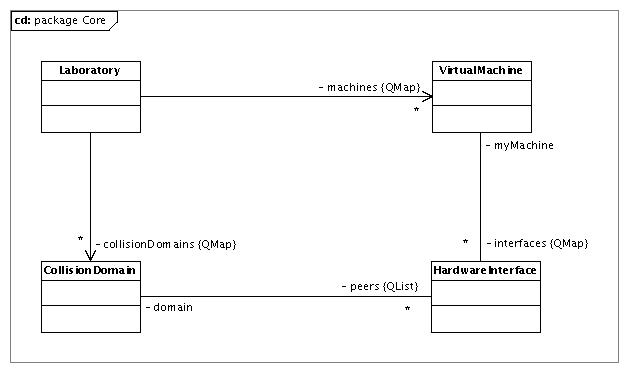
\includegraphics[width=12cm]{images/uml_package_core.png}
	\caption{Diagramma delle classi del package Core.}
	\label{figura:uml_package_core}
\end{figure}

Come si nota in figura \ref{figura:uml_package_core}, questo package ha una struttura molto semplice ma allo stesso tempo riesce a descrivere qualsiasi topologia di rete virtuale. Infatti, un laboratorio contiene un insieme di oggetti VirtualMachine e CollisionDomain contenuti all'interno di due Mappe ordinate per nome degli stessi. La giunzione tra questi ultimi due elementi è occupata dalla classe HardwareInterface che funge da collante di riferimento tra l'host virtuale, ed i vari domini di collisione a cui è collegato.
Grazie a questa semplice struttura \visualnetkit{} nasce da una parte come ambiente per la creazione di reti virtuali da emulare con \netkit{}, ma è potenzialmente in grado di essere riadattato in modo da poter produrre configurazioni per altri sistemi di emulazione.

Come vedremo più avanti, gli oggetti di tipo HardwareInterface saranno rappresentati da dei Links grafici all'interno della scena grafica.

\subsection{La gestione degli eventi}
Come in tutte le applicazioni software, ogni oggetto ha bisogno di essere ``gestito'' nel contesto dell'applicazione stessa.\\
La funzione di amministrazione e controllo del singolo oggetto, in applicazioni realizzate a regola d'arte, viene demandata ad altri oggetti tipicamente più leggeri ma non per questo meno complessi, detti \emph{handler}.

Le funzioni di controller sono state realizzate seguendo le linee guida del pattern \emph{Controller}\cite{AUPL04} ed assegnando le responsabilità responsabilità del controllo e della realizzazione di funzioni e compiti dell'oggetto interessato. In \visualnetkit{} esistono vari tipi di \emph{handlers}:
\begin{itemize}
\item \emph{Facade Controllers};
\item \emph{Use Case Controllers};
\item \emph{Mappers} - ossia macro elementi che disaccoppiano vista e dominio (introdotti più avanti in questo capitolo);
\item \emph{Property Controllers} - descritti più avanti in questo capitolo.
\end{itemize}

I \emph{Facade Controllers} vengono utilizzati per raccogliere le richeste che provengono dai livelli più alti - in particolare dagli \emph{Use Case Controllers} - quando c'è bisogno di una cecesso a basso livello che comporta un qualche tipo di cambiamento a livello di Dominio.

Gli \emph{Use Case Controllers}\footnote{Nella figura \ref{figura:vn_componenti} sono indicati come \emph{Handlers} generici.} sono posti in strati medio-alti dell'architettura e sono i primi oggetti che ricevono i segnali provenienti dall'interfaccia grafica. Questi effettuano una prima validazione dell'azione svolta e se non vi sono errori inoltrano la richiesta agli oggetti più bassi, in particolare ai \emph{Facade Controllers} e in qualche caso anche agli oggetti \emph{Mappers}.


\subsection{Interazione tra Utente e Proprietà degli Elementi}
Ogni elemento del dominio incapsula come di norma alcune proprietà di base. Queste, oltre a caratterizzare i vari oggetti, servono anche per descrivere una certa realtà di interesse espressa dall'utente; ciò significa che è proprio l'utente finale che vuole avere la possibilità di cambiare questi attributi.

Nel nostro caso abbiamo che oltre alle proprietà offerde dagli oggetti del dominio (ad esempio il nome di una \virtualmachine{}), per la natura modulare del sistema, è possibile che per un oggetto base vi siano collegati alcuni \plugin{} che offrono proprietà aggiuntive.\\
La gestione di queste è demandata ad oggetti (di tipo \emph{Use Case Controller}) che sono responsabili di renderizzare i dati, e ricevere le modifiche che l'utente desidera (si veda la figura \ref{figura:properties_uml1}). Come già descritto, questi oggetti vengono dinamicamente inseriti come handlers degli oggetti che rappresentano i dati delle properties, poichè la natura degli elementi che l'utente può selezionare è eterogenea; ogni tipologia di elemento possiede il suo \emph{Property Controller}.

\subsection{Gestione degli annullamenti: l'Undo Framework}
Per l'implementazione delle funzionalità di undo e di redo delle azioni svolte, è stato utilizzato un potente framework offerto da \qt{}. Questo sistema ha permesso, in fase realizzativa, di tralasciare molte dei dettagli implementativi e dirigere l'attenzione verso problematiche come la consistenza dei dati. Infatti, seppur le operazioni di undo o redo siano atomiche, esse interagiscono con lo strato dei \emph{Facade Controllers} e quindi indirettamente anche con gli oggetti del Dominio.

\subsubsection*{L'Undo Framework in \qt{}}
Il \emph{Qt Undo Framework} è un'implementazione del pattern \emph{Command}\cite{AUPL04}, per l'attuazione di funzionalità di undo/redo nelle applicazioni.\\
Il pattern \emph{Command} è basato sul concetto che tutte le funzioni di editing in un'applicazione siano realizzate con la creazione di istanze di oggetti command. Facendo il caso di un editor di testo, gli oggetti command applicano le modifiche al documento e sono memorizzati in uno stack dei comandi. Un \emph{QUndoCommand} rappresenta una singola azione di editing dello stato del documento; ad esempio, l'inserimento o l'eliminazione di blocchi di testo. Un comando può apportare cambiamenti al documento con azioni di \emph{redo()} o di \emph{undo()}.

Inoltre, ogni comando sa come annullare i cambiamenti da lui apportati e come riportare il documento allo stato precedente. Finché l'applicazione utilizza solo oggetti command per cambiare lo stato del documento, è possibile annullare una sequenza di comandi attraversando lo stack verso il basso e disfacendo ciascun comando. È anche possibile ripetere una sequenza di comandi percorrendo la pila all'inverso.

La flessibilità offerta da questo strumento è tale da poterla applicare ad ogni tipo di situazione. Analizziamo ora un esempio un po' più realistico e complesso.

Nel framework ogni azione che l'utente vuole poter annullare, è implementata in una classe che estende \emph{QUndoCommand}. Per ogni azione effettuata viene creato un apposito command che andrà inserito nel \emph{QUndoStack} di riferimento. Appena l'oggetto prende posto all'interno dello stack, la sua funzione di redo viene invocata per completare e/o effettuare l'azione richesta.

Il nostro esempio implementa un semplice diagramma grafico. È pertanto possibile eliminare e aggiungere elementi e muoverli tramite \emph{drag\&{}drop}. Ognuna di queste azioni possiede il corrispondente undo command che permette all'utente eventualmente di tornare sui suoi passi.
In figuara \ref{figura:qt_undo} è mostrato come un \emph{QUndoStack} può essere mostrato graficamente all'interno di un \emph{QUndoView}.

\begin{figure}[!htb]
	\centering
	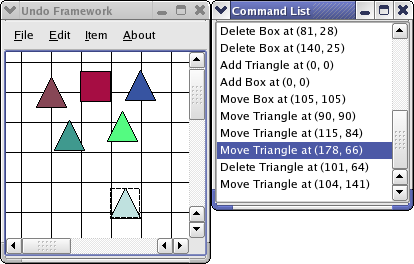
\includegraphics[width=10cm]{images/undoframeworkexample.png}
	\caption{Un esempio avanzato dell'Undo Framework offerdo da \qt{}.}
	\label{figura:qt_undo}
\end{figure}

\subsection{L'accesso al \fs{}}
Lo strato di persistenza dei dati nel complesso di ogni applicazione software, gioca un ruolo fondamentale. Generalmente posto nello strato più basso del sistema, questo elemento architetturale ha il duplice scopo di interagire con il \fs{} per salvare i dati inerenti alle varie configurazioni dell'applicazione e dei laboratory creati, nonché esportare questi ultimi in un formato accettato e riconosciuto dall'ambiente di emulazione desiderato.\\
Uno dei problemi riscontrati in fase di progettazione era come strutturare le informazioni che dovevano essere salvate. Da una parte occorreva salvare lo stato del laboratorio creato - in particolare lo stato del grafo della rete - mentre dall'altra parte occorreva trovare un buon sistema per poter esportare il laboratorio in modo da essere poi eseguito correttamente dal sistema di emulazione su cui quest'ambiente si basa\footnote{Ribadiamo il concetto che \visualnetkit{} nasce come ambiente per creazione di lab per \netkit{}, ma questo non vincola il tool ad un eventuale adattamento in favore di un qualsiasi altro sistema di emulazione.}.

Ad esempio, se un utente desidera salvare un lab per poi riaprirlo dev'essere possibile memorizzare metadati sugli elementi presenti nella scena grafica, quali potrebbero essere le posizioni degli oggetti stessi, delle etichette e informazioni inerenti ai \plugin{}.

Si è deciso di procedere, quindi, con la registrazione delle metainformazioni su di un file in formato \xml{}, nominato \emph{lab.xml} posto nella root directory del laboratorio.\\
Il fatto di salvare i metadati in un file separato rende il lab prodotto standard e auto descritto da un singolo file di configurazione esterno.
Un tag principale ``scene'' rappresenta alcune informazioni sulla scena grafica come ad esempio la dimensione. Internamente a questa vi sono tags di gruppo che descrivono i vari componenti grafici come links, aree, virtual machines e collision domains; ad ognuno sono associate informazioni extra che descrivono metadati aggiuntivi, quando previsto.

La vera e propria parte che esporta la struttura del laboratorio su \fs{} è stata divisa in quattro fasi:
\begin{description}
\item[Fase 1] questa fase iniziale è adibita alla creazione della struttura base delle directories, in particolare per ogni virtual machine presente nel lab creato, viene cerata una directory con il nome dell'host virtuale;
\item[Fase 2] è il momento della creazione del file \emph{lab.conf} che contiene la struttura fondamentale della rete a livello topologico, riconoscuta da \netkit{};
\item[Fase 3] questa fase è riservata al salvataggio dei file di ``sturtup'' delle macchine prenti\footnote{In \netkit{} ogni host virtuale che viene avviato può operare azioni di post-start grazie all'esecuzione del file \emph{.startup} inerente ad una precisa macchina virtuale.};
\item[Fase 4] l'ultimo step fa in modo che ogni plugin attivo possa offrire porzioni (o la totalità) di file di configurazioni che descrivono i propri settaggi.
\end{description}

\subsubsection*{Template Engine in \visualnetkit{}}
Nelle fasi due tre e quattro si è parlato della creazione dei file di configurazione; sia i \plugin{} che l'applicazione stessa utilizzano un sistema di \emph{mark-up} per la creaziene dei vari templates che andranno poi scritti dallo strato di persistenza all'interno dei files. Questi templates possiedono una struttura interna che prevede la sostituzione localizzata di alcune parti. Prendiamo in esame il templete che verrà utilizzato per creare il file ``lab.conf'':

\begin{figure}[!htb]
\begin{lstlisting}[language=csh]
###
# This file is createb by Visual Netkit <VISUAL_NETKIT_VERSION> version
# http://www.netkit.org ~ http://code.google.com/p/visual-netkit/
#

LAB_DESCRIPTION="<DESCRIPTION>"
LAB_VERSION="<VERSION>"
LAB_AUTHOR="<AUTHOR>"
LAB_EMAIL="<EMAIL>"
LAB_WEB="<WEB>"

<TOPOLOGY><HOST>[<ETH_NUMBER>]="<COLLISION_DOMAIN_NAME>"</TOPOLOGY>
\end{lstlisting}
\end{figure}
Il Template Engine interno all'applicazione viene invocato passando il riferimento (basato sul resource system di \qt{}) ad un template file. Questo viene prima caricato in memoria e successivamente vengono effettuare alcune sostituzioni di base come la sostituzione del \emph{mark-up}\\
``<VISUAL\_{}NETKIT\_{}VERSION>'' che viene sostituito dalla corrente versione del tool.
L'elemento che invoca il caricamento di un template riceve quindi il contenuto del file desiderato; successivamente vengono effettuate le altre sostituzioni tramite l'ausilio di espressioni regorali.\\
Osserviamo la riga $12$; l'oggetto incaricato di salvare il file ``lab.conf'' è incaricato di completare la struttura del file di configurazione inserendo la descrizione, la versione, l'autore, l'indirizzo email e il sito web del lab corrente, e successivamente costruirà la topologia dell'intera rete iterando tra i \emph{tag} ``<TOPOLOGY></TOPOLOGY>''.

In questo modo si riesce a creare un file di configurazione corretto e ben formattato come quello proposto qui sotto:

\begin{lstlisting}[language=csh]
###
# This file is createb by Visual Netkit 1.1 version
# http://www.netkit.org ~ http://code.google.com/p/visual-netkit/
#

LAB_DESCRIPTION="A simple laboratory"
LAB_VERSION="1.0"
LAB_AUTHOR="Alessio Di Fazio"
LAB_EMAIL="slux83@gmail.com"
LAB_WEB="http://code.google.com/p/visual-netkit/"

host1[0]="a"
host1[1]="b"

host2[0]="b"
host2[1]="c"

host3[0]="c"
host3[1]="d"
\end{lstlisting}
che descrive la topologia di rete presente in figura \ref{figura:vnetkit_graphics_view_1}.

È importante notare che il template dell'esempio appena citato risulti totalmetne indipendente dal motore di emulazione utilizzato, ed è dunque facilmente rimodellizzabile per essere adoperato con emulatori differenti.

Nel caso in cui un emulatore richiedesse una sintazzi particolare per le varie macchine virtuali, come ad esempio VNUML, basterebbe creare un semplice plugin che offra uno specifico template, ed aggungere questo plugin ai vari host virtuali presenti nella topologia di rete.

\subsection{Controllers tra Dominio e Vista}

\section{La gestione avanzata delle properties}
\subsection{Properties di base}
\subsection{Properties dei \plugin{}}

\section{Strumenti di supporto allo sviluppo}
\subsection{Il framework \qt{}}
\subsection{Altri strumenti secondari}
